\documentclass[12pt,a4paper]{article}
\usepackage[margin=1in]{geometry}
\usepackage{booktabs}
\usepackage{graphicx}
\usepackage{float}
\usepackage{amsmath}
\usepackage{caption}
\usepackage{hyperref}
\usepackage{setspace}
\usepackage{enumitem}
\captionsetup{font=small}
\onehalfspacing
\graphicspath{{figures/}}

\title{\textbf{5. EMPIRICAL FRAMEWORK}}
\author{Jordi Camps Triay}
\date{May 2026}

\begin{document}
\maketitle
\tableofcontents
\newpage

%======================================================================
% 5.1 VARIABLE SELECTION AND JUSTIFICATION
%======================================================================
\section{Variable Selection and Justification}

The empirical analysis requires two sets of variables: those that capture the structural conditions of the funding market (the independent variables) and those that capture the pricing of credit risk (the dependent variables). Data availability constrains the analysis: SOFR has been published only since April 2018, while corporate bond spreads and reserve balances are available from 2003 onward.

The following are the chosen variables:

\begin{enumerate}
  \item \textbf{Funding inputs.} SOFR--EFFR spread. The Secured Overnight Financing Rate minus the Effective Federal Funds Rate captures the price differential between secured (repo) and unsecured (federal funds) overnight borrowing.

  \item \textbf{Balance sheet quantities.} Reserve balances held at the Fed measure the aggregate quantity of settlement liquidity available to the banking system. As every payment between banks and repo transaction settles in reserves, their level determines whether the system operates in a regime of abundance or scarcity (Adrian and Shin, 2010). The Treasury General Account (TGA) balance captures fiscal cash flows that drain or inject reserves independently of monetary policy. The Overnight Reverse Repurchase (ON RRP) facility balance captures the voluntary liquidity parking by money market funds. Klee, Senyuz, and Yoldas (2021) document how the ON RRP facility acts as a ``borrower of last resort,'' absorbing excess liquidity when private repo rates approach the facility's offering rate; its usage surged from near zero to over \$2 trillion between 2021 and 2023, largely driven by drawdowns in the TGA and continued quantitative easing. Including the ON RRP balance tests whether this large-scale reallocation of money market fund portfolios---away from private repo lending and into the Fed's balance sheet---transmits to corporate credit pricing.

  \item \textbf{Credit spread variables.} Three measures capture the pricing of credit risk across the quality spectrum of investment-grade corporate bonds:
  \begin{enumerate}[label=(\alph*)]
    \item The Moody's Aaa corporate bond spread (Aaa yield minus the 10-year Treasury yield) measures the premium on the highest-quality corporate debt.
    \item The Moody's Baa corporate bond spread captures the premium on lower investment-grade bonds.
    \item The Baa--Aaa spread differential isolates the quality premium.
  \end{enumerate}

  \item \textbf{Risk appetite and global transmission variables.} The log ratio of HYG to LQD (high-yield and investment-grade bond ETFs) proxies for relative credit risk preference (Bauer, Bernanke and Milstein, 2023). The log ratio of HYG to SHV captures flight to quality. The nominal dollar index (DXY) captures the trade-weighted value of the dollar, which tends to strengthen when global dollar funding conditions tighten (Shin, 2012; Avdjiev et al., 2019). The iShares J.P. Morgan USD Emerging Markets Bond ETF (EMB) captures emerging-market sovereign credit conditions.
\end{enumerate}

\paragraph{Variables excluded.} The SOFR--OBFR spread was excluded due to near-perfect correlation with SOFR--EFFR ($\rho = 0.997$). The BGCR--TGCR spread was excluded because 97\% of its observations are exactly zero. The VIX and MOVE indices were excluded because they are outcome measures of aggregate market conditions rather than structural inputs to the funding system.


%======================================================================
% 5.2 DATA CONSTRUCTION AND PREPARATION
%======================================================================
\section{Data Construction and Preparation}

\subsection{Data sources}

\begin{table}[H]
\centering
\scalebox{0.82}{
\begin{tabular}{llll}
  \toprule
Variable & Source & Frequency & Start \\ 
  \midrule
SOFR & Federal Reserve Bank of New York & Daily & Apr 2018 \\ 
  EFFR & Federal Reserve (H.15) & Daily & Apr 2018 \\ 
  Baa corporate yield & FRED (Moody's) & Daily & May 2003 \\ 
  Aaa corporate yield & FRED (Moody's) & Daily & May 2003 \\ 
  10-year Treasury yield & FRED & Daily & May 2003 \\ 
  Reserve Balances & Federal Reserve (H.4.1) & Weekly (fwd-filled) & May 2003 \\ 
  TGA Balance & Federal Reserve (H.4.1) & Weekly (fwd-filled) & May 2003 \\ 
  ON RRP Balance & Federal Reserve Bank of New York & Daily & Mar 2014 \\ 
  DXY (Dollar Index) & Google Finance & Daily & Jan 2006 \\ 
  HYG (High Yield ETF) & Google Finance & Daily & Apr 2007 \\ 
  LQD (Inv. Grade ETF) & Google Finance & Daily & Jan 2005 \\ 
  SHV (Short Treasury ETF) & Google Finance & Daily & Jan 2007 \\ 
  EMB (EM Bond ETF) & Google Finance & Daily & Dec 2007 \\ 
   \bottomrule
\end{tabular}
}
\caption{Data Sources and Availability} 
\label{tab:data_sources}
\end{table}


Weekly series (Reserve Balances, TGA) are released on Wednesdays as part of the Federal Reserve's H.4.1 statistical release. Each Wednesday's value is forward-filled through the following business days until the next release (last-observation-carried-forward). Forward-filling introduces staleness, biasing against finding significant results at daily frequency; any significance found is therefore a conservative estimate.

Two sample periods are used. The \textbf{post-2018 sample} (April 2018--April 2026, $N \approx 2{,}004$) begins when the Federal Reserve Bank of New York started publishing SOFR and is used for Section~\ref{sec:granger}. The \textbf{dollar sample} (December 2007--April 2026, $N \approx 4{,}544$) uses the maximum overlap of all ETF variables and is used for Section~\ref{sec:dollar}.

\subsection{Stationarity and transformations}

A variable with a unit root will produce spurious regression results if included in levels. Table~\ref{tab:adf_all} presents the Augmented Dickey--Fuller test results, computed using the \texttt{ur.df()} function from the \texttt{urca} package (Pfaff, 2008). Level tests use the ``drift'' specification (constant, no deterministic trend); tests on returns and first differences use ``none'' (no deterministic components), following the standard approach for mean-zero financial returns. Augmentation lag order is selected by AIC over $\{0, \ldots, \lfloor(N{-}1)^{1/3}\rfloor\}$, and critical values are from MacKinnon (1996).

\begin{table}[H]
\centering
\scalebox{0.67}{
\begin{tabular}{lllrrrrrrl}
  \toprule
  Variable & Form & Sample & Lags & $N$ & ADF $\tau$ & 1\% c.v. & 5\% c.v. & 10\% c.v. & I(0)? \\ 
  \midrule
  \multicolumn{10}{l}{\textit{Panel A: Level tests}} \\ 
  \addlinespace
  SOFR--EFFR & Level & Post-2018 & 8 & 2004 & -8.33 & -3.43 & -2.86 & -2.57 & Yes \\ 
  Baa spread & Level & Post-2018 & 9 & 2002 & -3.35 & -3.43 & -2.86 & -2.57 & Yes \\ 
  Aaa spread & Level & Post-2018 & 12 & 2002 & -3.19 & -3.43 & -2.86 & -2.57 & Yes \\ 
  Baa--Aaa & Level & Post-2018 & 12 & 2002 & -2.85 & -3.43 & -2.86 & -2.57 & No \\ 
  Reserves & Level & Post-2018 & 5 & 2013 & -1.45 & -3.43 & -2.86 & -2.57 & No \\ 
  TGA & Level & Post-2018 & 10 & 2013 & -2.09 & -3.43 & -2.86 & -2.57 & No \\ 
  ON RRP & Level & Post-2018 & 8 & 2013 & -0.71 & -3.43 & -2.86 & -2.57 & No \\ 
  DXY & Level & 2008--2026 & 11 & 4527 & -1.38 & -3.43 & -2.86 & -2.57 & No \\ 
  log(HYG/LQD) & Level & 2008--2026 & 16 & 4527 & -2.75 & -3.43 & -2.86 & -2.57 & No \\ 
  log(HYG/SHV) & Level & 2008--2026 & 16 & 4527 & -3.17 & -3.43 & -2.86 & -2.57 & Yes \\ 
  EMB & Level & 2008--2026 & 8 & 4527 & -2.17 & -3.43 & -2.86 & -2.57 & No \\ 
  \addlinespace
  \multicolumn{10}{l}{\textit{Panel B: Analysis variables (transformed)}} \\ 
  \addlinespace
  Baa spread & First diff. & Post-2018 & 10 & 1991 & -11.15 & -2.58 & -1.95 & -1.62 & Yes \\ 
  Aaa spread & First diff. & Post-2018 & 11 & 1991 & -14.41 & -2.58 & -1.95 & -1.62 & Yes \\ 
  Baa--Aaa & First diff. & Post-2018 & 12 & 1991 & -10.93 & -2.58 & -1.95 & -1.62 & Yes \\ 
  Reserves & First diff. & Post-2018 & 4 & 2013 & -19.15 & -2.58 & -1.95 & -1.62 & Yes \\ 
  TGA & First diff. & Post-2018 & 9 & 2013 & -11.93 & -2.58 & -1.95 & -1.62 & Yes \\ 
  ON RRP & First diff. & Post-2018 & 7 & 2013 & -23.39 & -2.58 & -1.95 & -1.62 & Yes \\ 
  DXY & Log return & 2008--2026 & 10 & 4480 & -19.81 & -2.58 & -1.95 & -1.62 & Yes \\ 
  HYG/LQD & $\Delta$log ratio & 2008--2026 & 16 & 4500 & -17.49 & -2.58 & -1.95 & -1.62 & Yes \\ 
  HYG/SHV & $\Delta$log ratio & 2008--2026 & 16 & 4499 & -16.27 & -2.58 & -1.95 & -1.62 & Yes \\ 
  EMB & Log return & 2008--2026 & 16 & 4493 & -15.34 & -2.58 & -1.95 & -1.62 & Yes \\ 
  \bottomrule
\end{tabular}
}
\caption{Augmented Dickey--Fuller unit root tests. Panel~A tests variables in levels to establish integration order. Panel~B confirms stationarity of transformed variables entering the analysis. Level tests use the ``drift'' specification (constant, no trend); tests on returns and first differences use ``none'' (no deterministic components). Lag order selected by AIC over $\{0, \ldots, \lfloor(N{-}1)^{1/3}\rfloor\}$. Critical values from MacKinnon (1996).}
\label{tab:adf_all}
\end{table}


Panel~A establishes the integration order. The SOFR--EFFR spread is clearly stationary ($\tau = -8.33$). The Baa and Aaa spreads are stationary at the 5\% level but not at 1\%; the Baa--Aaa quality differential is borderline non-stationary ($\tau = -2.85$ vs.\ the 5\% critical value of $-2.86$). To be conservative, all three credit spread measures enter the Granger tests in first differences. Quantities (Reserves, TGA, ON RRP) are clearly non-stationary in levels and require first-differencing. For the dollar sample, DXY and EMB price levels contain unit roots; the log ratio of HYG to SHV is borderline stationary in levels ($\tau = -3.17$), while the HYG/LQD log ratio is non-stationary. Panel~B confirms that all transformed variables entering the analysis are stationary. DXY and EMB are expressed as log returns; the ETF ratios HYG/LQD and HYG/SHV are expressed as first differences of their log ratios (not log returns, since the ratio is not a cumulative price).

\subsection{SOFR--EFFR distribution and nonlinearity}

\begin{figure}[H]
\centering
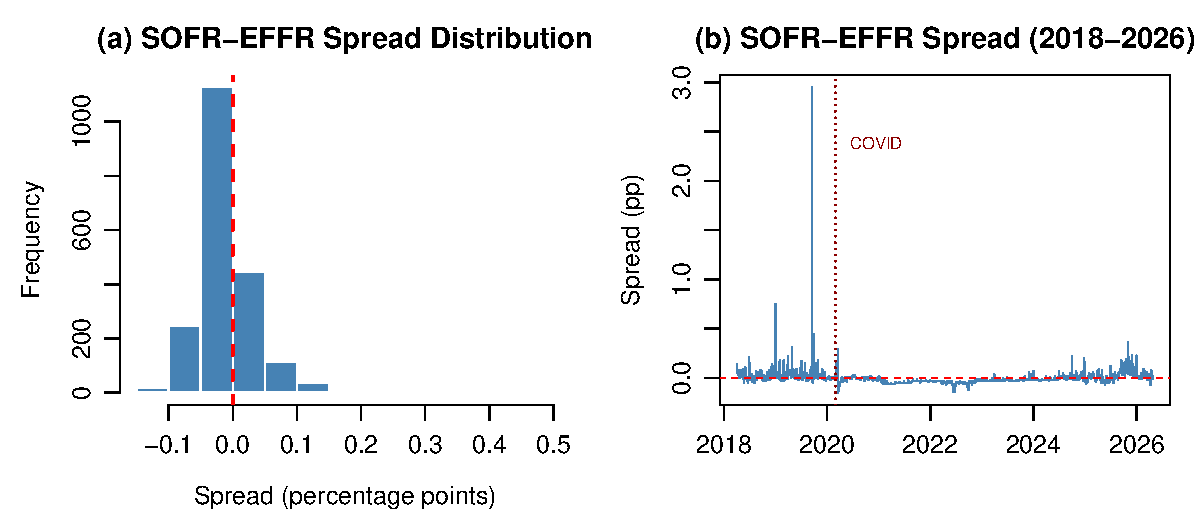
\includegraphics[width=0.95\textwidth]{fig_sofr_distribution.pdf}
\caption{Distribution and time series of the SOFR--EFFR spread (2018--2026). The spread is compressed at or near zero on approximately 88\% of trading days. The informational content is concentrated in discrete stress events (September 2019, March 2020), motivating the nonlinear interpretation discussed in Section~\ref{sec:granger}.}
\label{fig:sofr_dist}
\end{figure}


%======================================================================
% 5.3 PRICE AND COLLATERAL CHANNELS
%======================================================================
\section{Price and Collateral Channels on Credit Markets}
\label{sec:granger}

This section presents the Granger causality tests that constitute the first inferential step of the empirical analysis, with the aim of establish which of the chosen variables contain predictive information for credit spreads dynamics. Granger (1969) proposed that a variable $X$ is said to ``Granger-cause'' $Y$ if past values of $X$ contain information that helps predict $Y$ beyond $Y$'s own history. Rejection of the null hypothesis indicates that a lagged $X$ has statistically significant predictive content for $Y$ after controlling for $Y$'s own dynamics. However, it's important to emphasize that Granger causality establishes predictive precedence and not structural causation.

The bivariate Granger test evaluates:
\begin{align}
Y_t &= \alpha + \sum_{i=1}^{p} \beta_i Y_{t-i} + \sum_{i=1}^{p} \gamma_i X_{t-i} + \varepsilon_t \\
H_0&: \gamma_1 = \gamma_2 = \cdots = \gamma_p = 0 \quad \text{(no Granger causality)}
\end{align}

The analysis uses the post-2018 sample (April 2018--April 2026, $N \approx 2{,}004$ daily observations). Tests are conducted at $p \in \{1, 5, 10\}$ business days: lag~1 captures overnight transmission, lag~5 corresponds to one trading week (the typical settlement and rebalancing horizon in repo markets; Copeland, Martin, and Walker, 2014), and lag~10 (two trading weeks) captures slower portfolio adjustment effects. AIC and BIC lag selection for each bivariate pair is reported in Appendix~\ref{app:granger_robust}; for the key relationships, both criteria select lags within the $\{1, \ldots, 5\}$ range, confirming that our lag-5 specification lies within the information-criterion-preferred neighbourhood.

Given the pervasive conditional heteroskedasticity confirmed by ARCH-LM tests (Appendix~\ref{app:granger_robust}), all tables report both classical and HAC-robust $F$-statistics. The HAC covariance matrix uses the Quadratic Spectral kernel with bandwidth selected by the Andrews (1991) data-driven procedure, without prewhitening, as implemented in the \texttt{sandwich} package (Zeileis, 2004). The HAC-robust results are treated as the primary inference.

\subsection{Correlation diagnostics}

\begin{table}[H]
\centering
\scalebox{0.78}{
\begin{tabular}{rrrrrrr}
  \toprule
 & SOFR--EFFR & $\Delta$Baa & $\Delta$Aaa & $\Delta$(Baa--Aaa) & $\Delta$Reserves & $\Delta$TGA \\ 
  \midrule
SOFR--EFFR & 1.000 & 0.005 & 0.016 & -0.018 & -0.043 & 0.017 \\ 
  $\Delta$Baa & 0.005 & 1.000 & 0.744 & 0.122 & 0.020 & -0.014 \\ 
  $\Delta$Aaa & 0.016 & 0.744 & 1.000 & -0.573 & 0.017 & 0.053 \\ 
  $\Delta$(Baa--Aaa) & -0.018 & 0.122 & -0.573 & 1.000 & 0.000 & -0.096 \\ 
  $\Delta$Reserves & -0.043 & 0.020 & 0.017 & 0.000 & 1.000 & -0.350 \\ 
  $\Delta$TGA & 0.017 & -0.014 & 0.053 & -0.096 & -0.350 & 1.000 \\ 
   \bottomrule
\end{tabular}
}
\caption{Contemporaneous Correlation Matrix (Post-2018, Stationary Variables)} 
\label{tab:corr_post2018}
\end{table}


Two findings are relevant. First, SOFR--EFFR vs credit spread changes: the contemporaneous correlations are near zero ($r = 0.005$ for $\Delta$Baa, $r = 0.016$ for $\Delta$Aaa). Funding conditions and credit spreads do not move together on the same day. This does not mean they are unrelated, but perhaps means the transmission operates with a lag, which is exactly what Granger causality tests are designed to detect. Second, $\Delta$Reserves vs $\Delta$TGA: $r = -0.35$. This mechanical negative correlation reflects the Fed's balance sheet identity.

\subsection{Battery 1: Funding price channel}

\begin{table}[H]
\centering
\scalebox{0.72}{
\begin{tabular}{lrrrrlrrl}
  \toprule
Direction & Lag & $N$ & $F$ (class.) & $p$ (class.) &  & $F$ (HAC) & $p$ (HAC) &  \\ 
  \midrule
SOFR--EFFR $\rightarrow$ $\Delta$Baa & 1 & 2003 & 0.001 & 0.9763 &  & 0.001 & 0.9792 &  \\ 
  SOFR--EFFR $\rightarrow$ $\Delta$Aaa & 1 & 2003 & 0.890 & 0.3457 &  & 0.388 & 0.5336 &  \\ 
  SOFR--EFFR $\rightarrow$ $\Delta$(Baa--Aaa) & 1 & 2003 & 2.514 & 0.1130 &  & 0.998 & 0.3180 &  \\ 
  SOFR--EFFR $\rightarrow$ $\Delta$Baa & 5 & 1999 & 0.549 & 0.7394 &  & 2.731 & 0.0182 & * \\ 
  SOFR--EFFR $\rightarrow$ $\Delta$Aaa & 5 & 1999 & 1.163 & 0.3249 &  & 0.256 & 0.9371 &  \\ 
  SOFR--EFFR $\rightarrow$ $\Delta$(Baa--Aaa) & 5 & 1999 & 1.479 & 0.1933 &  & 2.041 & 0.0702 & . \\ 
  SOFR--EFFR $\rightarrow$ $\Delta$Baa & 10 & 1994 & 0.369 & 0.9600 &  & 2.241 & 0.0135 & * \\ 
  SOFR--EFFR $\rightarrow$ $\Delta$Aaa & 10 & 1994 & 0.810 & 0.6187 &  & 1.677 & 0.0806 & . \\ 
  SOFR--EFFR $\rightarrow$ $\Delta$(Baa--Aaa) & 10 & 1994 & 1.047 & 0.4006 &  & 3.635 & 0.0001 & *** \\ 
   \bottomrule
\end{tabular}
}
\caption{Battery 1: SOFR--EFFR $\rightarrow$ Credit Spread Changes (Post-2018)} 
\label{tab:price_post2018}
\end{table}


Under the classical $F$-test, the SOFR--EFFR spread shows no predictive power for any credit spread measure ($p > 0.11$ everywhere). However, the HAC-robust test reveals a more nuanced picture: SOFR--EFFR Granger-causes $\Delta$Baa at lags 5 and 10 ($p_{\text{HAC}} = 0.018, 0.014$) and $\Delta$(Baa--Aaa) at lag 10 ($p_{\text{HAC}} < 0.001$). The divergence between the two tests reflects the extreme conditional heteroskedasticity of the SOFR--EFFR spread: compressed at or near zero on approximately 88\% of trading days (skewness of 22.5), its rare spikes generate heteroskedastic residuals that distort classical standard errors in both directions. Given the near-degenerate distribution of the regressor, both tests have limited finite-sample reliability. Taken together with the rolling window evidence (Figure~\ref{fig:rolling_price}), these results suggest that the price channel operates episodically---activated during stress events rather than transmitting continuously.

\subsection{Battery 2: Funding quantity channel}

\begin{table}[H]
\centering
\scalebox{0.72}{
\begin{tabular}{lrrrrlrrl}
  \toprule
Direction & Lag & $N$ & $F$ (class.) & $p$ (class.) &  & $F$ (HAC) & $p$ (HAC) &  \\ 
  \midrule
SOFR--EFFR $\rightarrow$ $\Delta$Baa & 1 & 2003 & 0.001 & 0.9763 &  & 0.001 & 0.9792 &  \\ 
  SOFR--EFFR $\rightarrow$ $\Delta$Baa & 5 & 1999 & 0.549 & 0.7394 &  & 2.731 & 0.0182 & * \\ 
  SOFR--EFFR $\rightarrow$ $\Delta$Baa & 10 & 1994 & 0.369 & 0.9600 &  & 2.241 & 0.0135 & * \\ 
  SOFR--EFFR $\rightarrow$ $\Delta$Aaa & 1 & 2003 & 0.890 & 0.3457 &  & 0.388 & 0.5336 &  \\ 
  SOFR--EFFR $\rightarrow$ $\Delta$Aaa & 5 & 1999 & 1.163 & 0.3249 &  & 0.256 & 0.9371 &  \\ 
  SOFR--EFFR $\rightarrow$ $\Delta$Aaa & 10 & 1994 & 0.810 & 0.6187 &  & 1.677 & 0.0806 & . \\ 
  SOFR--EFFR $\rightarrow$ $\Delta$(Baa--Aaa) & 1 & 2003 & 2.514 & 0.1130 &  & 0.998 & 0.3180 &  \\ 
  SOFR--EFFR $\rightarrow$ $\Delta$(Baa--Aaa) & 5 & 1999 & 1.479 & 0.1933 &  & 2.041 & 0.0702 & . \\ 
  SOFR--EFFR $\rightarrow$ $\Delta$(Baa--Aaa) & 10 & 1994 & 1.047 & 0.4006 &  & 3.635 & 0.0001 & *** \\ 
  $\Delta$Reserves $\rightarrow$ $\Delta$Baa & 1 & 2003 & 1.781 & 0.1822 &  & 1.154 & 0.2829 &  \\ 
  $\Delta$Reserves $\rightarrow$ $\Delta$Baa & 5 & 1999 & 1.628 & 0.1493 &  & 1.192 & 0.3104 &  \\ 
  $\Delta$Reserves $\rightarrow$ $\Delta$Baa & 10 & 1994 & 1.548 & 0.1166 &  & 1.230 & 0.2662 &  \\ 
  $\Delta$Reserves $\rightarrow$ $\Delta$Aaa & 1 & 2003 & 6.830 & 0.0090 & ** & 3.032 & 0.0818 & . \\ 
  $\Delta$Reserves $\rightarrow$ $\Delta$Aaa & 5 & 1999 & 3.493 & 0.0038 & ** & 1.999 & 0.0758 & . \\ 
  $\Delta$Reserves $\rightarrow$ $\Delta$Aaa & 10 & 1994 & 2.219 & 0.0145 & * & 1.432 & 0.1599 &  \\ 
  $\Delta$Reserves $\rightarrow$ $\Delta$(Baa--Aaa) & 1 & 2003 & 6.741 & 0.0095 & ** & 2.108 & 0.1467 &  \\ 
  $\Delta$Reserves $\rightarrow$ $\Delta$(Baa--Aaa) & 5 & 1999 & 2.537 & 0.0268 & * & 1.393 & 0.2238 &  \\ 
  $\Delta$Reserves $\rightarrow$ $\Delta$(Baa--Aaa) & 10 & 1994 & 1.439 & 0.1569 &  & 1.343 & 0.2017 &  \\ 
  $\Delta$TGA $\rightarrow$ $\Delta$Baa & 1 & 2003 & 3.249 & 0.0716 & . & 2.191 & 0.1390 &  \\ 
  $\Delta$TGA $\rightarrow$ $\Delta$Baa & 5 & 1999 & 1.141 & 0.3365 &  & 1.020 & 0.4041 &  \\ 
  $\Delta$TGA $\rightarrow$ $\Delta$Baa & 10 & 1994 & 0.604 & 0.8120 &  & 0.606 & 0.8099 &  \\ 
  $\Delta$TGA $\rightarrow$ $\Delta$Aaa & 1 & 2003 & 1.537 & 0.2152 &  & 2.229 & 0.1356 &  \\ 
  $\Delta$TGA $\rightarrow$ $\Delta$Aaa & 5 & 1999 & 1.326 & 0.2503 &  & 1.203 & 0.3054 &  \\ 
  $\Delta$TGA $\rightarrow$ $\Delta$Aaa & 10 & 1994 & 0.923 & 0.5111 &  & 0.853 & 0.5776 &  \\ 
  $\Delta$TGA $\rightarrow$ $\Delta$(Baa--Aaa) & 1 & 2003 & 2.800 & 0.0944 & . & 1.702 & 0.1922 &  \\ 
  $\Delta$TGA $\rightarrow$ $\Delta$(Baa--Aaa) & 5 & 1999 & 3.743 & 0.0022 & ** & 1.157 & 0.3281 &  \\ 
  $\Delta$TGA $\rightarrow$ $\Delta$(Baa--Aaa) & 10 & 1994 & 2.506 & 0.0054 & ** & 1.002 & 0.4395 &  \\ 
  $\Delta$ON RRP $\rightarrow$ $\Delta$Baa & 1 & 2003 & 0.691 & 0.4058 &  & 0.592 & 0.4417 &  \\ 
  $\Delta$ON RRP $\rightarrow$ $\Delta$Baa & 5 & 1999 & 1.129 & 0.3425 &  & 1.034 & 0.3957 &  \\ 
  $\Delta$ON RRP $\rightarrow$ $\Delta$Baa & 10 & 1994 & 0.721 & 0.7050 &  & 0.905 & 0.5273 &  \\ 
  $\Delta$ON RRP $\rightarrow$ $\Delta$Aaa & 1 & 2003 & 1.258 & 0.2621 &  & 1.085 & 0.2977 &  \\ 
  $\Delta$ON RRP $\rightarrow$ $\Delta$Aaa & 5 & 1999 & 0.492 & 0.7823 &  & 0.586 & 0.7111 &  \\ 
  $\Delta$ON RRP $\rightarrow$ $\Delta$Aaa & 10 & 1994 & 0.913 & 0.5204 &  & 1.437 & 0.1578 &  \\ 
  $\Delta$ON RRP $\rightarrow$ $\Delta$(Baa--Aaa) & 1 & 2003 & 0.278 & 0.5982 &  & 0.234 & 0.6284 &  \\ 
  $\Delta$ON RRP $\rightarrow$ $\Delta$(Baa--Aaa) & 5 & 1999 & 0.797 & 0.5517 &  & 0.927 & 0.4620 &  \\ 
  $\Delta$ON RRP $\rightarrow$ $\Delta$(Baa--Aaa) & 10 & 1994 & 0.890 & 0.5417 &  & 0.990 & 0.4502 &  \\ 
   \bottomrule
\end{tabular}
}
\caption{Granger Causality: Funding $\rightarrow$ Credit Spreads (Post-2018)} 
\label{tab:granger_fwd_post2018}
\end{table}


From these results, four findings stand out:

\begin{enumerate}
  \item \textbf{Reserve changes predict Aaa spread changes, but significance weakens under HAC.} The classical $F$-test finds $\Delta$Reserves $\rightarrow$ $\Delta$Aaa significant at all lags ($p = 0.009, 0.004, 0.015$). Under HAC-robust inference, the relationship retains only marginal significance at lags 1 and 5 ($p_{\text{HAC}} = 0.082, 0.076$) and becomes insignificant at lag 10 ($p_{\text{HAC}} = 0.16$). The classical $F$-statistics are inflated by the pervasive conditional heteroskedasticity documented in the residual diagnostics (Appendix~\ref{app:granger_robust}).

  \item \textbf{Reserve changes do not predict Baa spread changes.} $\Delta$Reserves $\rightarrow$ $\Delta$Baa is insignificant under both classical ($p = 0.18, 0.15, 0.12$) and HAC inference ($p_{\text{HAC}} = 0.28, 0.31, 0.27$). Aaa-rated bonds are closer substitutes for Treasuries in repo collateral and are therefore more sensitive to changes in aggregate reserve balances. This pattern is consistent with the safe-asset substitution channel documented by Krishnamurthy and Vissing-Jorgensen (2012), who show that Aaa corporate bonds carry a convenience yield that varies with the supply of Treasury-like safe assets.

  \item \textbf{TGA changes predict the Baa--Aaa quality differential under classical inference only.} The classical $F$-test finds $\Delta$TGA $\rightarrow$ $\Delta$(Baa--Aaa) significant at lags 5 and 10 ($p = 0.002, 0.005$), but HAC-robust inference eliminates this significance entirely ($p_{\text{HAC}} = 0.33, 0.44$). The fiscal plumbing channel described by Duffie and Krishnamurthy (2016) may still operate, but the statistical evidence at daily frequency is not robust to heteroskedasticity correction.

  \item \textbf{ON RRP shows no predictive power.} Changes in Overnight Reverse Repurchase Agreements fail to Granger-cause any credit spread measure under both classical ($p > 0.26$) and HAC ($p > 0.16$) inference. Despite the theoretical motivation---Klee, Senyuz, and Yoldas (2021) show that the ON RRP facility absorbed over \$2 trillion in money market fund liquidity that might otherwise have flowed into private repo and short-term credit markets---the empirical result is unambiguous. The mechanism is institutionally segmented: money market funds that use the ON RRP facility are restricted by SEC Rule~2a-7 to high-quality, short-duration instruments and have no direct access to corporate bond markets. The liquidity ``parked'' at the Fed therefore substitutes for Treasury bills, agency debt, and private repo---not for investment-grade corporate credit. Any transmission from ON RRP to Baa or Aaa spreads would require an indirect chain (ON RRP $\rightarrow$ repo rates $\rightarrow$ dealer balance sheets $\rightarrow$ corporate bonds), which the Granger test at daily frequency lacks the power to detect.
\end{enumerate}

\subsection{Battery 3: Reverse causality checks}

\begin{table}[H]
\centering
\scalebox{0.72}{
\begin{tabular}{lrrrrlrrl}
  \toprule
Direction & Lag & $N$ & $F$ (class.) & $p$ (class.) &  & $F$ (HAC) & $p$ (HAC) &  \\ 
  \midrule
$\Delta$Baa $\rightarrow$ SOFR--EFFR & 1 & 2003 & 0.122 & 0.7274 &  & 0.162 & 0.6874 &  \\ 
  $\Delta$Baa $\rightarrow$ SOFR--EFFR & 5 & 1999 & 0.614 & 0.6891 &  & 1.272 & 0.2733 &  \\ 
  $\Delta$Baa $\rightarrow$ SOFR--EFFR & 10 & 1994 & 0.449 & 0.9223 &  & 0.916 & 0.5175 &  \\ 
  $\Delta$Baa $\rightarrow$ $\Delta$Reserves & 1 & 2003 & 0.043 & 0.8362 &  & 0.027 & 0.8690 &  \\ 
  $\Delta$Baa $\rightarrow$ $\Delta$Reserves & 5 & 1999 & 4.631 & 0.0003 & *** & 1.361 & 0.2362 &  \\ 
  $\Delta$Baa $\rightarrow$ $\Delta$Reserves & 10 & 1994 & 3.694 & 0.0001 & *** & 1.368 & 0.1889 &  \\ 
  $\Delta$Baa $\rightarrow$ $\Delta$TGA & 1 & 2003 & 4.697 & 0.0303 & * & 3.702 & 0.0545 & . \\ 
  $\Delta$Baa $\rightarrow$ $\Delta$TGA & 5 & 1999 & 1.499 & 0.1868 &  & 1.253 & 0.2818 &  \\ 
  $\Delta$Baa $\rightarrow$ $\Delta$TGA & 10 & 1994 & 1.788 & 0.0579 & . & 1.720 & 0.0709 & . \\ 
  $\Delta$Aaa $\rightarrow$ SOFR--EFFR & 1 & 2003 & 0.038 & 0.8448 &  & 0.057 & 0.8108 &  \\ 
  $\Delta$Aaa $\rightarrow$ SOFR--EFFR & 5 & 1999 & 0.628 & 0.6781 &  & 1.214 & 0.3002 &  \\ 
  $\Delta$Aaa $\rightarrow$ SOFR--EFFR & 10 & 1994 & 0.537 & 0.8648 &  & 0.703 & 0.7220 &  \\ 
  $\Delta$Aaa $\rightarrow$ $\Delta$Reserves & 1 & 2003 & 0.000 & 0.9833 &  & 0.000 & 0.9898 &  \\ 
  $\Delta$Aaa $\rightarrow$ $\Delta$Reserves & 5 & 1999 & 3.499 & 0.0037 & ** & 1.518 & 0.1809 &  \\ 
  $\Delta$Aaa $\rightarrow$ $\Delta$Reserves & 10 & 1994 & 3.502 & 0.0001 & *** & 1.632 & 0.0918 & . \\ 
  $\Delta$Aaa $\rightarrow$ $\Delta$TGA & 1 & 2003 & 7.104 & 0.0078 & ** & 4.517 & 0.0337 & * \\ 
  $\Delta$Aaa $\rightarrow$ $\Delta$TGA & 5 & 1999 & 2.927 & 0.0123 & * & 2.121 & 0.0602 & . \\ 
  $\Delta$Aaa $\rightarrow$ $\Delta$TGA & 10 & 1994 & 3.002 & 0.0009 & *** & 2.168 & 0.0173 & * \\ 
   \bottomrule
\end{tabular}
}
\caption{Reverse Causality: Credit Spreads $\rightarrow$ Funding (Post-2018)} 
\label{tab:granger_rev_post2018}
\end{table}


The reverse causality tests show an important divergence between classical and HAC inference. Under classical $F$-tests, $\Delta$Baa and $\Delta$Aaa both predict $\Delta$Reserves at lags 5 and 10 (all $p < 0.004$), and $\Delta$Aaa predicts $\Delta$TGA at all lags ($p = 0.008, 0.012, 0.001$). However, HAC-robust inference substantially reduces this apparent feedback: credit $\rightarrow$ reserves significance disappears ($p_{\text{HAC}} > 0.18$ everywhere), and credit $\rightarrow$ TGA survives only for $\Delta$Aaa $\rightarrow$ $\Delta$TGA at lags 1 and 10 ($p_{\text{HAC}} = 0.034, 0.017$). Credit spread changes do not predict the SOFR--EFFR spread under either test ($p > 0.27$ uniformly). The reduction in reverse causality under HAC mitigates the bidirectional feedback concern that complicates causal interpretation of the forward-direction results.

\subsection{Rolling window analysis}

\begin{figure}[H]
\centering
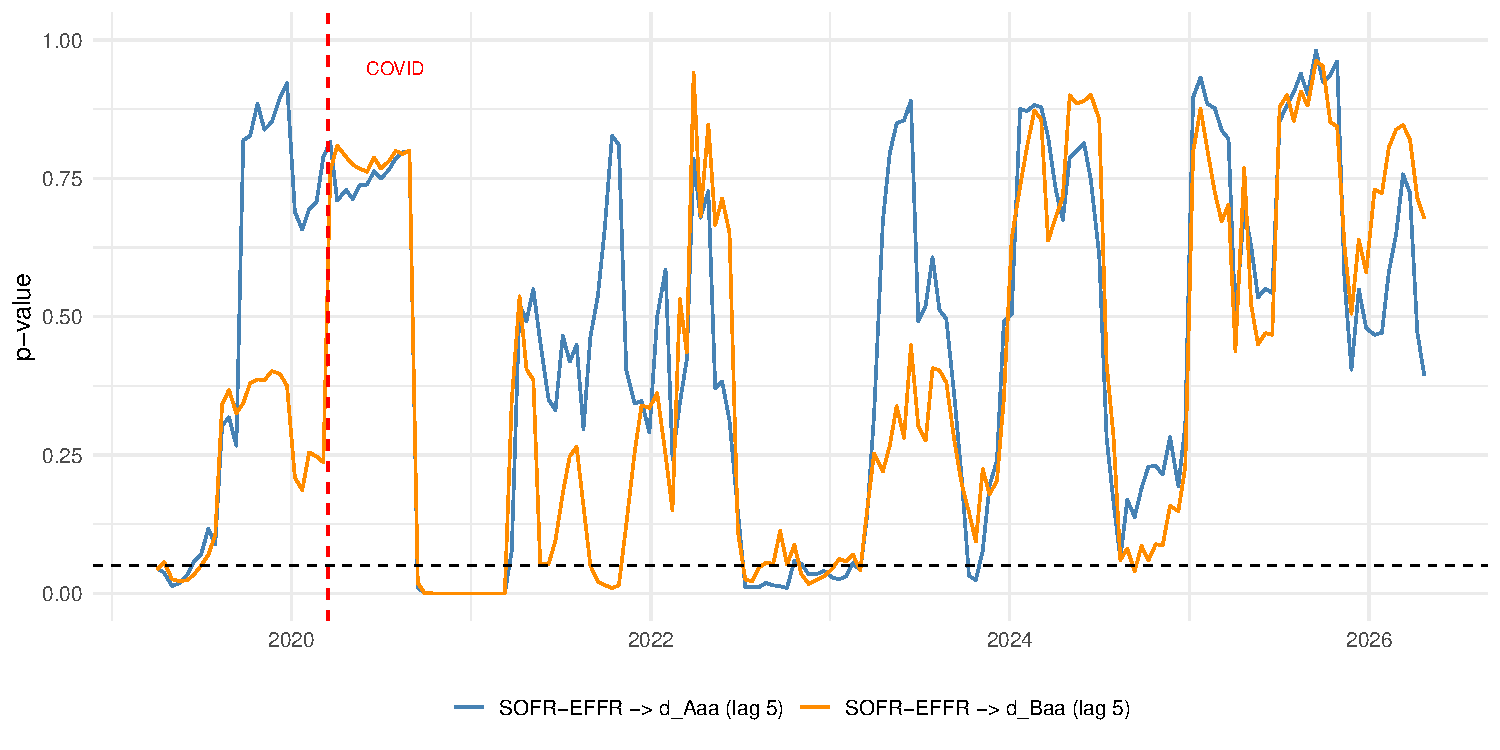
\includegraphics[width=0.95\textwidth]{fig_a5_rolling_granger.pdf}
\caption{Rolling Granger $p$-values (250-day window, lag 5) for SOFR--EFFR predicting credit spread changes. The dashed black line marks the 5\% significance threshold. Predictive power activates episodically during stress episodes.}
\label{fig:rolling_price}
\end{figure}

\begin{figure}[H]
\centering
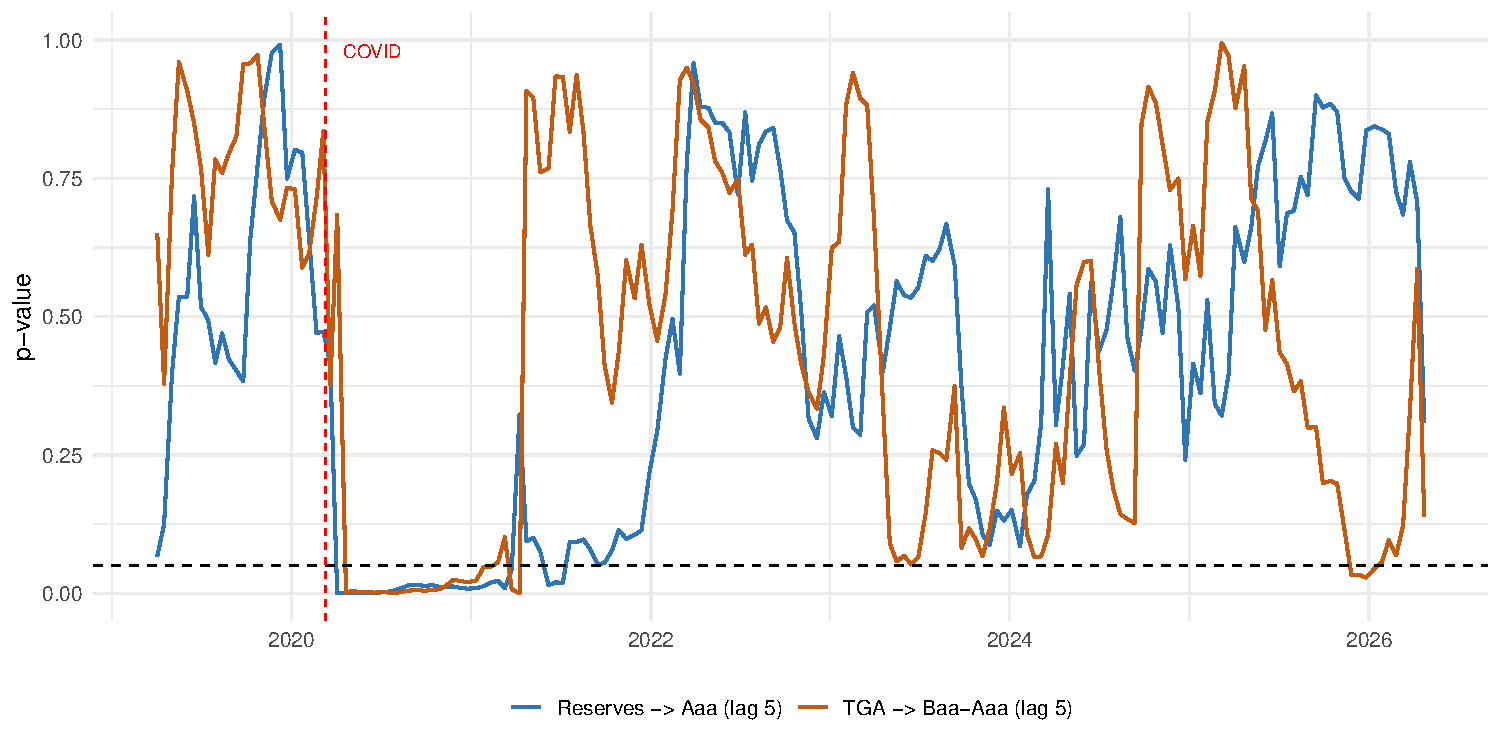
\includegraphics[width=0.95\textwidth]{fig_a6_rolling_granger_qty.pdf}
\caption{Rolling Granger $p$-values (250-day window, lag 5) for quantity channel: $\Delta$Reserves $\rightarrow$ $\Delta$Aaa and $\Delta$TGA $\rightarrow$ $\Delta$(Baa--Aaa). Significance concentrates during stress windows.}
\label{fig:rolling_qty}
\end{figure}

The rolling window analysis (250-day window, lag 5) reveals the time-varying nature of predictive relationships. The SOFR--EFFR price channel (Figure~\ref{fig:rolling_price}) shows brief windows of significance around the March 2020 COVID shock and the September 2019 repo crisis. The quantity channel (Figure~\ref{fig:rolling_qty}) shows a different pattern: $\Delta$Reserves $\rightarrow$ $\Delta$Aaa drops below the 5\% threshold during and after the COVID episode, while $\Delta$TGA $\rightarrow$ $\Delta$(Baa--Aaa) exhibits episodic significance that aligns with periods of active Treasury cash management. The concentration of significance in specific stress windows supports the interpretation that the funding--credit transmission is regime-dependent.

Robustness checks---including residual diagnostics (Breusch--Godfrey, ARCH-LM), COVID sensitivity, and lag selection---are reported in Appendix~\ref{app:granger_robust}.


%======================================================================
% 5.4 DOLLAR CHANNEL
%======================================================================
\section{Dollar Channel in Credit Markets}
\label{sec:dollar}

The previous section established that funding quantities Granger-cause credit spread movements through a collateral channel, while the SOFR--EFFR price channel operates episodically during stress episodes. This section complements that analysis by examining the role of the US dollar as a barometer of global risk appetite and its influence on credit markets.

The theoretical motivation draws on the growing literature linking the dollar to global financial conditions. Having access to limited data has constrained the analysis (e.g.\ cross-currency basis swaps have not been used). However, these mechanisms predict that dollar appreciation should be associated with: (i) a decline in the relative price of risky credit assets (HYG) versus investment-grade (LQD) or safe assets (SHV), reflecting reduced risk appetite; and (ii) a decline in emerging market bond prices (EMB), reflecting the tightening of dollar funding conditions for EM borrowers (Gonz\'alez-Hermosillo, 2008).

These predictions are tested using three dependent variables constructed from ETF prices:

\begin{itemize}
  \item \textbf{HYG/LQD ratio} (risk appetite): A decline signals increased risk aversion within credit markets.
  \item \textbf{HYG/SHV ratio} (flight to quality): A decline signals a flight from risky credit to safe government securities.
  \item \textbf{EMB} (emerging market credit): A decline reflects tightening dollar funding conditions and/or increased sovereign risk premia.
\end{itemize}

The analysis also examines whether nominal dollar movements (DXY hereon) are linked to Federal Reserve balance sheet quantities ($\Delta$Reserves, $\Delta$TGA), connecting the dollar channel to the domestic funding plumbing analyzed in the previous section.

\subsection{Data and methodology}

The sample spans December 2007 to April 2026 ($N \approx 4{,}544$ daily observations), determined by the latest start date among the four ETFs (EMB, launched December 2007). DXY and EMB are expressed as daily log returns; the ETF ratios HYG/LQD and HYG/SHV are expressed as first differences of their log ratios. Stationarity of all transformed variables is confirmed in Table~\ref{tab:adf_all} (Panel~B).

\begin{table}[H]
\centering
\begin{tabular}{lrrrrrrr}
  \toprule
Variable & N & Mean & SD & Skew & Kurt & Min & Max \\ 
  \midrule
$r_{\text{DXY}}$ (\%) & 4497 & 0.00596 & 0.35291 & -0.07 & 7.10 & -2.5620 & 1.8964 \\
  $r$(HYG/LQD) & 4517 & -0.00006 & 0.00671 & -0.34 & 25.67 & -0.0875 & 0.0844 \\
  $r$(HYG/SHV) & 4516 & -0.00003 & 0.00704 & 0.44 & 45.43 & -0.0840 & 0.1227 \\
  $r_{\text{EMB}}$ (\%) & 4510 & -0.00026 & 0.69073 & -1.96 & 41.24 & -10.6587 & 6.5128 \\ 
   \bottomrule
\end{tabular}
\caption{Summary Statistics: Daily Log Returns (2008--2026)} 
\label{tab:sumstats_dollar}
\end{table}


Table~\ref{tab:sumstats_dollar} reports summary statistics. All four series exhibit excess kurtosis well above the Gaussian benchmark of 3, with EMB returns showing extreme leptokurtosis (kurtosis = 41.2) driven by the March 2020 crash.

\begin{table}[H]
\centering
\begin{tabular}{rrrrr}
  \toprule
 & DXY & HYG/LQD & HYG/SHV & EMB \\ 
  \midrule
DXY & 1.000 & -0.240 & -0.377 & -0.353 \\ 
  HYG/LQD & -0.240 & 1.000 & 0.661 & 0.125 \\ 
  HYG/SHV & -0.377 & 0.661 & 1.000 & 0.490 \\ 
  EMB & -0.353 & 0.125 & 0.490 & 1.000 \\ 
   \bottomrule
\end{tabular}
\caption{Contemporaneous Correlation Matrix (Daily Log Returns)} 
\label{tab:corr_dollar}
\end{table}


The correlation matrix (Table~\ref{tab:corr_dollar}) confirms the expected negative association between dollar returns and all three credit measures. The strongest contemporaneous correlation is between DXY and HYG/SHV ($\rho \approx -0.38$), followed by EMB ($\rho \approx -0.35$) and HYG/LQD ($\rho \approx -0.24$).

We apply the same Granger causality framework and HAC-robust inference described in Section~\ref{sec:granger}.

\subsection{Results}

\begin{figure}[H]
\centering
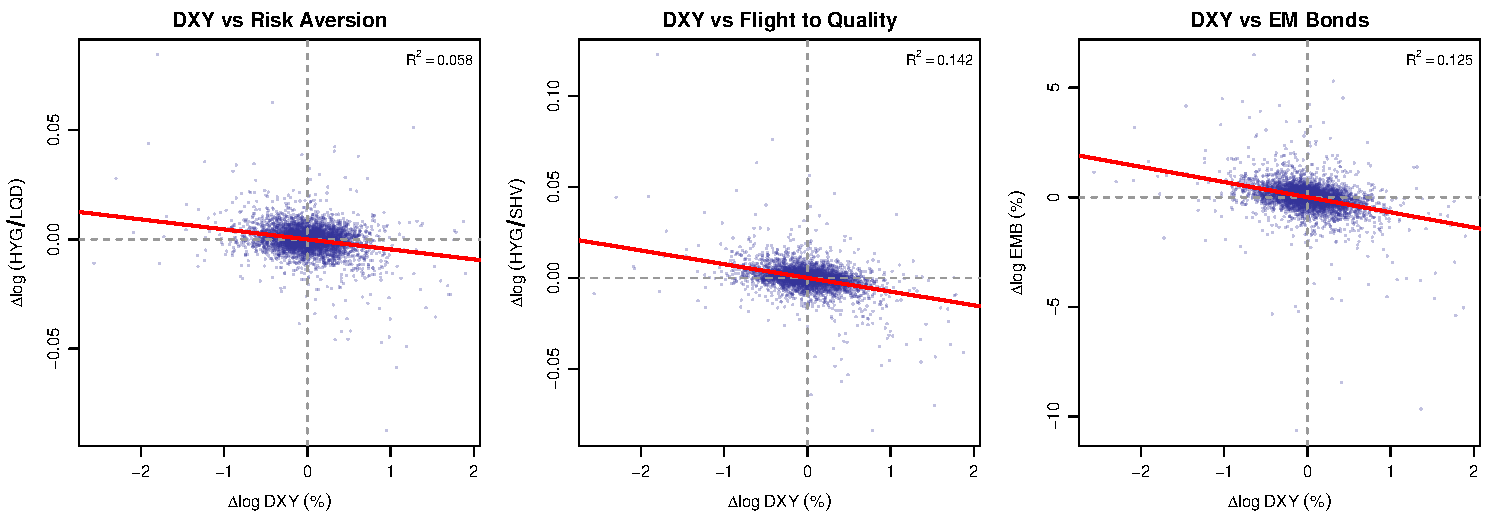
\includegraphics[width=0.95\textwidth]{fig_scatter_dxy.pdf}
\caption{Scatter plots of daily DXY log returns against each credit measure (2008--2026). All three relationships are negative. $R^2$ values range from 5.8\% (HYG/LQD) to 14.2\% (HYG/SHV).}
\label{fig:scatter_dxy}
\end{figure}

\paragraph{Battery 1: Dollar predicts credit measures.}

\begin{table}[H]
\centering
\scalebox{0.72}{
\begin{tabular}{lrrrrlrrl}
  \toprule
Direction & Lag & $N$ & $F$ (class.) & $p$ (class.) &  & $F$ (HAC) & $p$ (HAC) &  \\ 
  \midrule
$r$ DXY $\rightarrow$ $r$(HYG/LQD) & 1 & 4492 & 2.469 & 0.1162 &  & 0.901 & 0.3425 &  \\ 
  $r$ DXY $\rightarrow$ $r$(HYG/LQD) & 5 & 4488 & 6.712 & 0.0000 & *** & 2.362 & 0.0376 & * \\ 
  $r$ DXY $\rightarrow$ $r$(HYG/LQD) & 10 & 4483 & 3.952 & 0.0000 & *** & 1.579 & 0.1063 &  \\ 
  $r$ DXY $\rightarrow$ $r$(HYG/SHV) & 1 & 4491 & 5.561 & 0.0184 & * & 3.223 & 0.0727 & . \\ 
  $r$ DXY $\rightarrow$ $r$(HYG/SHV) & 5 & 4487 & 10.585 & 0.0000 & *** & 2.696 & 0.0194 & * \\ 
  $r$ DXY $\rightarrow$ $r$(HYG/SHV) & 10 & 4482 & 6.810 & 0.0000 & *** & 1.795 & 0.0562 & . \\ 
  $r$ DXY $\rightarrow$ $r$ EMB & 1 & 4485 & 50.983 & 0.0000 & *** & 14.504 & 0.0001 & *** \\ 
  $r$ DXY $\rightarrow$ $r$ EMB & 5 & 4481 & 14.041 & 0.0000 & *** & 3.182 & 0.0072 & ** \\ 
  $r$ DXY $\rightarrow$ $r$ EMB & 10 & 4476 & 8.417 & 0.0000 & *** & 2.936 & 0.0011 & ** \\ 
   \bottomrule
\end{tabular}
}
\caption{Granger Causality: DXY $\rightarrow$ Credit/Risk Measures (2008--2026)} 
\label{tab:gc_dxy_credit}
\end{table}


The results reveal a clear hierarchy of predictive power:

\begin{itemize}
  \item \textbf{DXY $\rightarrow$ EMB}: The strongest result. Under HAC-robust inference, DXY Granger-causes EMB returns at all three lag orders ($p = 0.0001$ at lag 1, $p = 0.007$ at lag 5, $p = 0.001$ at lag 10). This result is consistent with the Bruno and Shin (2015) channel: dollar appreciation tightens funding conditions for EM borrowers with dollar-denominated debt.

  \item \textbf{DXY $\rightarrow$ HYG/SHV}: Dollar returns predict the flight-to-quality ratio at lag 5 ($p_{\text{HAC}} = 0.019$), with marginal significance at lags 1 and 10 ($p = 0.073$ and $0.056$).

  \item \textbf{DXY $\rightarrow$ HYG/LQD}: The weakest channel. Significant only at lag 5 under HAC ($p = 0.038$). HYG/LQD captures only the within-credit rotation (high-yield vs.\ investment-grade), whereas HYG/SHV also captures the cross-asset-class rotation into Treasuries.
\end{itemize}

\paragraph{Battery 2: Reverse causality.}

\begin{table}[H]
\centering
\scalebox{0.72}{
\begin{tabular}{lrrrrlrrl}
  \toprule
Direction & Lag & $N$ & $F$ (class.) & $p$ (class.) &  & $F$ (HAC) & $p$ (HAC) &  \\ 
  \midrule
$r$(HYG/LQD) $\rightarrow$ $r$ DXY & 1 & 4492 & 4.376 & 0.0365 & * & 2.113 & 0.1461 &  \\ 
  $r$(HYG/LQD) $\rightarrow$ $r$ DXY & 5 & 4488 & 1.636 & 0.1468 &  & 0.698 & 0.6252 &  \\ 
  $r$(HYG/LQD) $\rightarrow$ $r$ DXY & 10 & 4483 & 2.626 & 0.0035 & ** & 1.056 & 0.3934 &  \\ 
  $r$(HYG/SHV) $\rightarrow$ $r$ DXY & 1 & 4491 & 67.132 & 0.0000 & *** & 12.812 & 0.0003 & *** \\ 
  $r$(HYG/SHV) $\rightarrow$ $r$ DXY & 5 & 4487 & 14.554 & 0.0000 & *** & 3.105 & 0.0084 & ** \\ 
  $r$(HYG/SHV) $\rightarrow$ $r$ DXY & 10 & 4482 & 8.023 & 0.0000 & *** & 3.104 & 0.0006 & *** \\ 
  $r$ EMB $\rightarrow$ $r$ DXY & 1 & 4485 & 43.482 & 0.0000 & *** & 10.727 & 0.0011 & ** \\ 
  $r$ EMB $\rightarrow$ $r$ DXY & 5 & 4481 & 12.205 & 0.0000 & *** & 3.984 & 0.0013 & ** \\ 
  $r$ EMB $\rightarrow$ $r$ DXY & 10 & 4476 & 8.485 & 0.0000 & *** & 3.052 & 0.0007 & *** \\ 
   \bottomrule
\end{tabular}
}
\caption{Granger Causality: Credit/Risk Measures $\rightarrow$ DXY (Reverse, 2008--2026)} 
\label{tab:gc_credit_dxy}
\end{table}


The reverse causality tests reveal substantial bidirectional feedback:

\begin{itemize}
  \item \textbf{HYG/SHV $\rightarrow$ DXY}: Significant at all lags ($p_{\text{HAC}} = 0.0003, 0.008, 0.0006$). The flight-to-quality ratio captures risk-off shifts that simultaneously strengthen the dollar through safe-haven demand for US assets.

  \item \textbf{EMB $\rightarrow$ DXY}: Also significant at all lags ($p_{\text{HAC}} = 0.001, 0.001, 0.0007$). Emerging market stress feeds back to dollar strength through capital repatriation and dollar demand.

  \item \textbf{HYG/LQD $\rightarrow$ DXY}: Not significant under HAC ($p > 0.14$ at all lags). Within-credit rotations (HYG vs.\ LQD) do not carry information about global dollar dynamics.
\end{itemize}

The strong bidirectional causality between DXY and EMB/HYG--SHV is consistent with the reflexive nature of the global financial cycle described by Rey (2013) and Bruno and Shin (2015).

\paragraph{Battery 3: DXY and balance sheet quantities.}

\begin{table}[H]
\centering
\scalebox{0.72}{
\begin{tabular}{lrrrrlrrl}
  \toprule
Direction & Lag & $N$ & $F$ (class.) & $p$ (class.) &  & $F$ (HAC) & $p$ (HAC) &  \\ 
  \midrule
$\Delta$Reserves $\rightarrow$ $r$ DXY & 1 & 4496 & 8.205 & 0.0042 & ** & 4.221 & 0.0400 & * \\ 
  $\Delta$Reserves $\rightarrow$ $r$ DXY & 5 & 4492 & 1.909 & 0.0895 & . & 1.056 & 0.3830 &  \\ 
  $\Delta$Reserves $\rightarrow$ $r$ DXY & 10 & 4487 & 1.653 & 0.0857 & . & 1.211 & 0.2784 &  \\ 
  $\Delta$TGA $\rightarrow$ $r$ DXY & 1 & 4496 & 0.065 & 0.7984 &  & 0.056 & 0.8136 &  \\ 
  $\Delta$TGA $\rightarrow$ $r$ DXY & 5 & 4492 & 0.982 & 0.4271 &  & 1.119 & 0.3481 &  \\ 
  $\Delta$TGA $\rightarrow$ $r$ DXY & 10 & 4487 & 0.929 & 0.5051 &  & 1.005 & 0.4361 &  \\ 
  $r$ DXY $\rightarrow$ $\Delta$Reserves & 1 & 4496 & 1.408 & 0.2354 &  & 1.395 & 0.2377 &  \\ 
  $r$ DXY $\rightarrow$ $\Delta$Reserves & 5 & 4492 & 0.548 & 0.7400 &  & 0.655 & 0.6580 &  \\ 
  $r$ DXY $\rightarrow$ $\Delta$Reserves & 10 & 4487 & 1.587 & 0.1037 &  & 1.534 & 0.1206 &  \\ 
  $r$ DXY $\rightarrow$ $\Delta$TGA & 1 & 4496 & 4.221 & 0.0400 & * & 4.575 & 0.0325 & * \\ 
  $r$ DXY $\rightarrow$ $\Delta$TGA & 5 & 4492 & 1.421 & 0.2131 &  & 1.622 & 0.1506 &  \\ 
  $r$ DXY $\rightarrow$ $\Delta$TGA & 10 & 4487 & 1.552 & 0.1148 &  & 1.282 & 0.2341 &  \\ 
   \bottomrule
\end{tabular}
}
\caption{Granger Causality: DXY $\leftrightarrow$ Reserves, TGA (2008--2026)} 
\label{tab:gc_dxy_qty}
\end{table}


Results show weaker significance. Changes in reserves are marginally significant at lag 1 ($p_{\text{HAC}} = 0.04$) for DXY but not at longer lags; DXY movements are significant at lag 1 ($p_{\text{HAC}} = 0.033$) for changes in TGA but not at longer lags. The weak linkage suggests that the dollar channel operates largely independently of the domestic funding quantity channel.

\subsection{Rolling Granger analysis}

\begin{figure}[H]
\centering
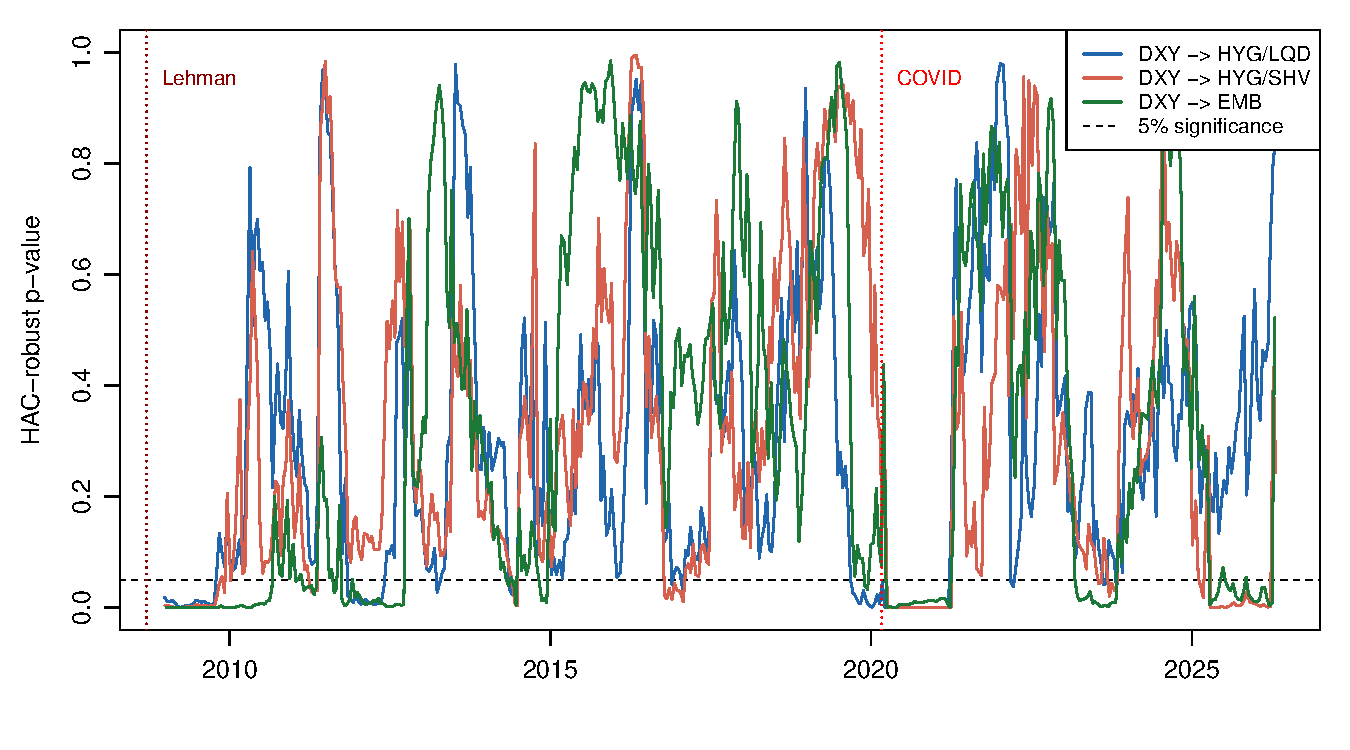
\includegraphics[width=0.95\textwidth]{fig_rolling_granger_dxy.pdf}
\caption{Rolling Granger $p$-values (250-day window, lag 5) for DXY predicting each credit measure. DXY $\rightarrow$ EMB shows the most persistent predictive power. The 250-day window corresponds to one trading year, matching the rolling correlation horizon (Forbes and Rigobon, 2002) and providing approximately 23 observations per parameter for the 11-parameter lag-5 specification.}
\label{fig:rolling_granger_dxy}
\end{figure}

\subsection{Rolling correlation analysis}

\begin{figure}[H]
\centering
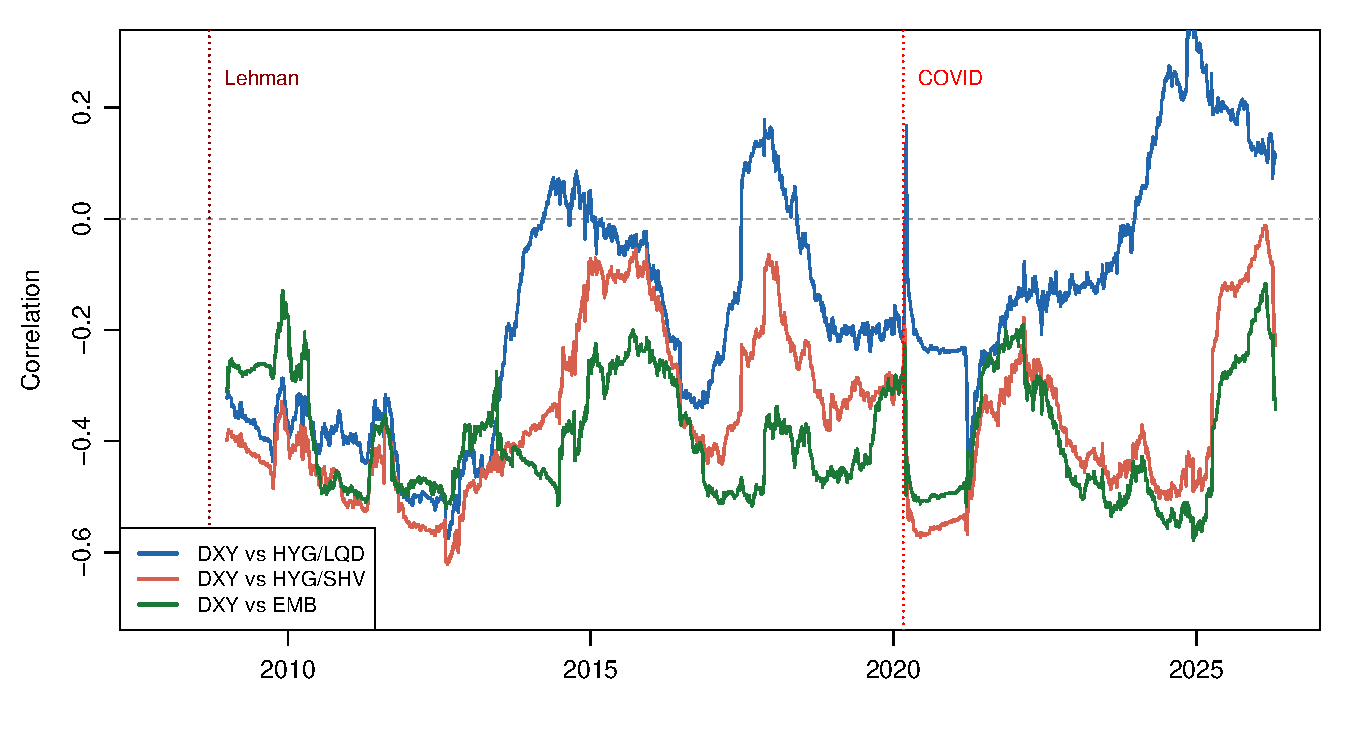
\includegraphics[width=0.95\textwidth]{fig_rolling_corr_dxy.pdf}
\caption{250-day rolling correlation between daily DXY returns and each credit measure (2008--2026). We use a 250-day rolling window, corresponding to approximately one trading year---a standard choice in the time-varying correlation literature (Forbes and Rigobon, 2002).}
\label{fig:rolling_corr_dxy}
\end{figure}

The DXY--EMB correlation is the most stable and persistently negative ($-0.3$ to $-0.6$), reflecting the structural nature of the dollar channel for emerging-market borrowers. DXY--HYG/SHV is mostly negative ($-0.2$ to $-0.5$), weakening during calm periods. DXY--HYG/LQD is not uniform; positive episodes (2015--2016 and 2023--2025) occur when dollar strength coincided with a risk-on environment.

Robustness checks for the dollar analysis---including lag selection, residual diagnostics, and COVID sensitivity---are reported in Appendix~\ref{app:dollar_robust}.


%======================================================================
% APPENDICES
%======================================================================
\newpage
\appendix

%----------------------------------------------------------------------
\section{Robustness: Price and Collateral Channels (Section~\ref{sec:granger})}
\label{app:granger_robust}

\subsection{Lag selection}

\begin{table}[H]
\centering
\caption{Information Criterion Lag Selection for Bivariate Granger Pairs (Post-2018)} 
\label{tab:lag_selection}
\scalebox{0.82}{
\begin{tabular}{llrrr}
  \toprule
$X$ & $Y$ & AIC lag & BIC lag & $N$ \\ 
  \midrule
SOFR--EFFR & $\Delta$Baa & 2 & 2 & 2004 \\ 
  $\Delta$Reserves & $\Delta$Baa & 2 & 2 & 2004 \\ 
  $\Delta$TGA & $\Delta$Baa & 2 & 2 & 2004 \\ 
  $\Delta$ON RRP & $\Delta$Baa & 2 & 2 & 2004 \\ 
  SOFR--EFFR & $\Delta$Aaa & 4 & 1 & 2004 \\ 
  $\Delta$Reserves & $\Delta$Aaa & 4 & 1 & 2004 \\ 
  $\Delta$TGA & $\Delta$Aaa & 2 & 1 & 2004 \\ 
  $\Delta$ON RRP & $\Delta$Aaa & 2 & 1 & 2004 \\ 
  SOFR--EFFR & $\Delta$(Baa--Aaa) & 3 & 1 & 2004 \\ 
  $\Delta$Reserves & $\Delta$(Baa--Aaa) & 3 & 3 & 2004 \\ 
  $\Delta$TGA & $\Delta$(Baa--Aaa) & 3 & 3 & 2004 \\ 
  $\Delta$ON RRP & $\Delta$(Baa--Aaa) & 3 & 1 & 2004 \\ 
  $\Delta$Baa & SOFR--EFFR & 9 & 9 & 2004 \\ 
  $\Delta$Aaa & SOFR--EFFR & 9 & 9 & 2004 \\ 
  $\Delta$Baa & $\Delta$Reserves & 15 & 15 & 2004 \\ 
  $\Delta$Aaa & $\Delta$Reserves & 15 & 15 & 2004 \\ 
  $\Delta$Baa & $\Delta$TGA & 15 & 15 & 2004 \\ 
  $\Delta$Aaa & $\Delta$TGA & 15 & 15 & 2004 \\ 
   \bottomrule
\end{tabular}
}
\end{table}


\subsection{Residual diagnostics}

\begin{table}[H]
\centering
\caption{Residual Diagnostics: Breusch-Godfrey (order 5) and ARCH-LM (order 5) Tests} 
\label{tab:diagnostics}
\scalebox{0.78}{
\begin{tabular}{lrrrlrrl}
  \toprule
Direction & Lag & BG stat & BG $p$ & BG reject? & ARCH-LM & ARCH $p$ & ARCH reject? \\ 
  \midrule
$\Delta$Reserves $\rightarrow$ $\Delta$Aaa & 1 & 25.097 & 0.0001 & Yes & 589.437 & 0.0000 & Yes \\ 
  $\Delta$Reserves $\rightarrow$ $\Delta$Aaa & 5 & 3.536 & 0.6180 & No & 540.546 & 0.0000 & Yes \\ 
  $\Delta$Reserves $\rightarrow$ $\Delta$Aaa & 10 & 23.375 & 0.0003 & Yes & 544.523 & 0.0000 & Yes \\ 
  $\Delta$Reserves $\rightarrow$ $\Delta$(Baa--Aaa) & 1 & 39.666 & 0.0000 & Yes & 387.328 & 0.0000 & Yes \\ 
  $\Delta$Reserves $\rightarrow$ $\Delta$(Baa--Aaa) & 5 & 8.943 & 0.1114 & No & 348.155 & 0.0000 & Yes \\ 
  $\Delta$TGA $\rightarrow$ $\Delta$(Baa--Aaa) & 5 & 8.669 & 0.1230 & No & 384.844 & 0.0000 & Yes \\ 
  $\Delta$TGA $\rightarrow$ $\Delta$(Baa--Aaa) & 10 & 24.448 & 0.0002 & Yes & 404.221 & 0.0000 & Yes \\ 
  SOFR--EFFR $\rightarrow$ $\Delta$Baa & 1 & 39.539 & 0.0000 & Yes & 163.885 & 0.0000 & Yes \\ 
  SOFR--EFFR $\rightarrow$ $\Delta$Baa & 5 & 12.617 & 0.0272 & Yes & 131.647 & 0.0000 & Yes \\ 
   \bottomrule
\end{tabular}
}
\end{table}


The Breusch--Godfrey test rejects the null of no serial correlation at order 5 for several lag-1 specifications but not for the lag-5 specifications, suggesting that sufficient lagged dependent variables absorb most of the serial dependence. The ARCH-LM test rejects overwhelmingly ($p < 0.001$) for every specification, confirming pervasive conditional heteroskedasticity. This reinforces the importance of HAC-robust inference.

\subsection{COVID-19 sensitivity}

\begin{table}[H]
\centering
\caption{COVID Robustness: Granger Causality With and Without February--May 2020} 
\label{tab:covid}
\scalebox{0.7}{
\begin{tabular}{llrrrrl}
  \toprule
Sample & Direction & Lag & $N$ & $F$-stat & $p$-value &  \\ 
  \midrule
Full & $\Delta$Reserves $\rightarrow$ $\Delta$Aaa & 1 & 2004 & 6.830 & 0.0090 & *** \\ 
  Full & $\Delta$Reserves $\rightarrow$ $\Delta$Aaa & 5 & 2004 & 3.493 & 0.0038 & *** \\ 
  Full & $\Delta$Reserves $\rightarrow$ $\Delta$Aaa & 10 & 2004 & 2.219 & 0.0145 & ** \\ 
  Full & $\Delta$Reserves $\rightarrow$ $\Delta$Baa & 1 & 2004 & 1.781 & 0.1822 &  \\ 
  Full & $\Delta$Reserves $\rightarrow$ $\Delta$Baa & 5 & 2004 & 1.628 & 0.1493 &  \\ 
  Full & $\Delta$Reserves $\rightarrow$ $\Delta$Baa & 10 & 2004 & 1.548 & 0.1166 &  \\ 
  Full & $\Delta$Reserves $\rightarrow$ $\Delta$(Baa--Aaa) & 1 & 2004 & 6.741 & 0.0095 & *** \\ 
  Full & $\Delta$Reserves $\rightarrow$ $\Delta$(Baa--Aaa) & 5 & 2004 & 2.537 & 0.0268 & ** \\ 
  Full & $\Delta$Reserves $\rightarrow$ $\Delta$(Baa--Aaa) & 10 & 2004 & 1.439 & 0.1569 &  \\ 
  Full & $\Delta$TGA $\rightarrow$ $\Delta$(Baa--Aaa) & 1 & 2004 & 2.800 & 0.0944 & * \\ 
  Full & $\Delta$TGA $\rightarrow$ $\Delta$(Baa--Aaa) & 5 & 2004 & 3.743 & 0.0022 & *** \\ 
  Full & $\Delta$TGA $\rightarrow$ $\Delta$(Baa--Aaa) & 10 & 2004 & 2.506 & 0.0054 & *** \\ 
  Full & $\Delta$TGA $\rightarrow$ $\Delta$Baa & 1 & 2004 & 3.249 & 0.0716 & * \\ 
  Full & $\Delta$TGA $\rightarrow$ $\Delta$Baa & 5 & 2004 & 1.141 & 0.3365 &  \\ 
  Full & $\Delta$TGA $\rightarrow$ $\Delta$Baa & 10 & 2004 & 0.604 & 0.8120 &  \\ 
  Full & SOFR--EFFR $\rightarrow$ $\Delta$Baa & 1 & 2004 & 0.001 & 0.9763 &  \\ 
  Full & SOFR--EFFR $\rightarrow$ $\Delta$Baa & 5 & 2004 & 0.549 & 0.7394 &  \\ 
  Full & SOFR--EFFR $\rightarrow$ $\Delta$Baa & 10 & 2004 & 0.369 & 0.9600 &  \\ 
  Full & SOFR--EFFR $\rightarrow$ $\Delta$Aaa & 1 & 2004 & 0.890 & 0.3457 &  \\ 
  Full & SOFR--EFFR $\rightarrow$ $\Delta$Aaa & 5 & 2004 & 1.163 & 0.3249 &  \\ 
  Full & SOFR--EFFR $\rightarrow$ $\Delta$Aaa & 10 & 2004 & 0.810 & 0.6187 &  \\ 
  Excl. COVID & $\Delta$Reserves $\rightarrow$ $\Delta$Aaa & 1 & 1923 & 0.539 & 0.4631 &  \\ 
  Excl. COVID & $\Delta$Reserves $\rightarrow$ $\Delta$Aaa & 5 & 1923 & 1.173 & 0.3199 &  \\ 
  Excl. COVID & $\Delta$Reserves $\rightarrow$ $\Delta$Aaa & 10 & 1923 & 0.829 & 0.6004 &  \\ 
  Excl. COVID & $\Delta$Reserves $\rightarrow$ $\Delta$Baa & 1 & 1923 & 0.312 & 0.5767 &  \\ 
  Excl. COVID & $\Delta$Reserves $\rightarrow$ $\Delta$Baa & 5 & 1923 & 1.479 & 0.1935 &  \\ 
  Excl. COVID & $\Delta$Reserves $\rightarrow$ $\Delta$Baa & 10 & 1923 & 1.116 & 0.3456 &  \\ 
  Excl. COVID & $\Delta$Reserves $\rightarrow$ $\Delta$(Baa--Aaa) & 1 & 1923 & 1.204 & 0.2727 &  \\ 
  Excl. COVID & $\Delta$Reserves $\rightarrow$ $\Delta$(Baa--Aaa) & 5 & 1923 & 0.393 & 0.8542 &  \\ 
  Excl. COVID & $\Delta$Reserves $\rightarrow$ $\Delta$(Baa--Aaa) & 10 & 1923 & 0.784 & 0.6445 &  \\ 
  Excl. COVID & $\Delta$TGA $\rightarrow$ $\Delta$(Baa--Aaa) & 1 & 1923 & 0.498 & 0.4807 &  \\ 
  Excl. COVID & $\Delta$TGA $\rightarrow$ $\Delta$(Baa--Aaa) & 5 & 1923 & 2.121 & 0.0602 & * \\ 
  Excl. COVID & $\Delta$TGA $\rightarrow$ $\Delta$(Baa--Aaa) & 10 & 1923 & 1.533 & 0.1215 &  \\ 
  Excl. COVID & $\Delta$TGA $\rightarrow$ $\Delta$Baa & 1 & 1923 & 0.238 & 0.6255 &  \\ 
  Excl. COVID & $\Delta$TGA $\rightarrow$ $\Delta$Baa & 5 & 1923 & 0.749 & 0.5871 &  \\ 
  Excl. COVID & $\Delta$TGA $\rightarrow$ $\Delta$Baa & 10 & 1923 & 0.426 & 0.9348 &  \\ 
  Excl. COVID & SOFR--EFFR $\rightarrow$ $\Delta$Baa & 1 & 1923 & 1.219 & 0.2696 &  \\ 
  Excl. COVID & SOFR--EFFR $\rightarrow$ $\Delta$Baa & 5 & 1923 & 0.597 & 0.7023 &  \\ 
  Excl. COVID & SOFR--EFFR $\rightarrow$ $\Delta$Baa & 10 & 1923 & 0.395 & 0.9496 &  \\ 
  Excl. COVID & SOFR--EFFR $\rightarrow$ $\Delta$Aaa & 1 & 1923 & 0.427 & 0.5135 &  \\ 
  Excl. COVID & SOFR--EFFR $\rightarrow$ $\Delta$Aaa & 5 & 1923 & 0.083 & 0.9949 &  \\ 
  Excl. COVID & SOFR--EFFR $\rightarrow$ $\Delta$Aaa & 10 & 1923 & 0.270 & 0.9876 &  \\ 
   \bottomrule
\end{tabular}
}
\end{table}


Under classical inference, $\Delta$Reserves $\rightarrow$ $\Delta$Aaa loses all significance when the February--May 2020 period is excluded ($p = 0.46, 0.32, 0.60$ at lags 1, 5, and 10). The $\Delta$TGA $\rightarrow$ $\Delta$(Baa--Aaa) relationship also weakens, though it retains marginal significance at lag~5.

This finding shapes the economic interpretation: the reserves--credit transmission is not a constant relationship---it is an \emph{episodic mechanism that activates during extreme stress}. The rolling window analysis (Figures~\ref{fig:rolling_price} and~\ref{fig:rolling_qty}) visually confirms this pattern.

\subsection{Multiple testing}

Across all three batteries, we conduct 54 individual Granger tests under both classical and HAC-robust inference. At the 5\% significance level, random chance alone would produce roughly 2.7 rejections per test type. Under HAC (the primary inference), five tests reject at 5\%: the SOFR--EFFR price channel at longer lags and $\Delta$Aaa $\rightarrow$ $\Delta$TGA in the reverse battery. Two features argue against spurious discovery. First, significance clusters in economically coherent pairs rather than appearing randomly across specifications: reserves predict Aaa but not Baa (consistent with the safe-asset substitution channel; Krishnamurthy and Vissing-Jorgensen, 2012), and the price channel operates episodically at longer lags rather than uniformly. Second, the divergence between classical and HAC results is itself informative: it reveals which relationships survive correction for the pervasive conditional heteroskedasticity documented in the residual diagnostics.


%----------------------------------------------------------------------
\section{Robustness: Dollar Channel (Section~\ref{sec:dollar})}
\label{app:dollar_robust}

\subsection{Lag selection}

\begin{table}[H]
\centering
\begin{tabular}{llrrr}
  \toprule
$X$ & $Y$ & AIC lag & BIC lag & $N$ \\ 
  \midrule
$r$ DXY & $r$(HYG/LQD) & 11 & 3 & 4493 \\ 
  $r$ DXY & $r$(HYG/SHV) & 15 & 1 & 4492 \\ 
  $r$ DXY & $r$ EMB & 14 & 6 & 4486 \\ 
  $r$(HYG/LQD) & $r$ DXY & 11 & 3 & 4493 \\ 
  $r$(HYG/SHV) & $r$ DXY & 15 & 1 & 4492 \\ 
  $r$ EMB & $r$ DXY & 14 & 6 & 4486 \\ 
  $\Delta$Reserves & $r$ DXY & 11 & 1 & 4497 \\ 
  $\Delta$TGA & $r$ DXY & 10 & 5 & 4497 \\ 
  $r$ DXY & $\Delta$Reserves & 11 & 1 & 4497 \\ 
  $r$ DXY & $\Delta$TGA & 10 & 5 & 4497 \\ 
   \bottomrule
\end{tabular}
\caption{Information Criterion Lag Selection for Bivariate Granger Pairs (Dollar Sample)} 
\label{tab:lag_selection_dollar}
\end{table}


BIC selects lag 1 for most quantity pairs and lags 1--6 for the credit pairs, while AIC selects longer lags (10--15). Our choice of testing at lags 1, 5, and 10 spans the range recommended by both criteria.

\subsection{Residual diagnostics}

\begin{table}[H]
\centering
\scalebox{0.72}{
\begin{tabular}{lrrrlrrl}
  \toprule
Direction & Lag & BG stat & BG $p$ & BG reject? & ARCH-LM & ARCH $p$ & ARCH reject? \\ 
  \midrule
$r$ DXY $\rightarrow$ $r$(HYG/LQD) & 1 & 70.862 & 0.0000 & Yes & 648.408 & 0.0000 & Yes \\ 
  $r$ DXY $\rightarrow$ $r$(HYG/LQD) & 5 & 2.050 & 0.8422 & No & 699.355 & 0.0000 & Yes \\ 
  $r$ DXY $\rightarrow$ $r$(HYG/SHV) & 1 & 34.472 & 0.0000 & Yes & 692.044 & 0.0000 & Yes \\ 
  $r$ DXY $\rightarrow$ $r$(HYG/SHV) & 5 & 9.458 & 0.0921 & No & 704.394 & 0.0000 & Yes \\ 
  $r$ DXY $\rightarrow$ $r$ EMB & 1 & 24.769 & 0.0002 & Yes & 609.619 & 0.0000 & Yes \\ 
  $r$ DXY $\rightarrow$ $r$ EMB & 5 & 121.530 & 0.0000 & Yes & 573.646 & 0.0000 & Yes \\ 
  $\Delta$Reserves $\rightarrow$ $r$ DXY & 1 & 4.186 & 0.5229 & No & 348.869 & 0.0000 & Yes \\ 
  $\Delta$Reserves $\rightarrow$ $r$ DXY & 5 & 16.016 & 0.0068 & Yes & 354.310 & 0.0000 & Yes \\ 
  $\Delta$TGA $\rightarrow$ $r$ DXY & 1 & 4.602 & 0.4663 & No & 339.668 & 0.0000 & Yes \\ 
  $\Delta$TGA $\rightarrow$ $r$ DXY & 5 & 17.264 & 0.0040 & Yes & 340.627 & 0.0000 & Yes \\ 
  $r$ DXY $\rightarrow$ $\Delta$TGA & 1 & 278.046 & 0.0000 & Yes & 231.475 & 0.0000 & Yes \\ 
  $r$ DXY $\rightarrow$ $\Delta$TGA & 5 & 24.979 & 0.0001 & Yes & 210.781 & 0.0000 & Yes \\ 
   \bottomrule
\end{tabular}
}
\caption{Residual Diagnostics: Breusch-Godfrey (order 5) and ARCH-LM (order 5) Tests} 
\label{tab:diagnostics_dollar}
\end{table}


The Breusch--Godfrey test (order 5) rejects the null of no serial correlation for several lag-1 specifications but generally not for lag-5 specifications. The ARCH-LM test rejects ($p < 0.001$) for every specification, confirming pervasive conditional heteroskedasticity. This reinforces the importance of HAC-robust inference used throughout.

\subsection{COVID-19 sensitivity}

\begin{table}[H]
\centering
\scalebox{0.75}{
\begin{tabular}{llrrrrl}
  \toprule
Sample & Direction & Lag & $N$ & $F$ (HAC) & $p$ (HAC) &  \\ 
  \midrule
Full & $r$ DXY $\rightarrow$ $r$(HYG/LQD) & 1 & 4492 & 0.901 & 0.3425 &  \\ 
  Full & $r$ DXY $\rightarrow$ $r$(HYG/LQD) & 5 & 4488 & 2.362 & 0.0376 & * \\ 
  Full & $r$ DXY $\rightarrow$ $r$(HYG/LQD) & 10 & 4483 & 1.579 & 0.1063 &  \\ 
  Full & $r$ DXY $\rightarrow$ $r$(HYG/SHV) & 1 & 4491 & 3.223 & 0.0727 & . \\ 
  Full & $r$ DXY $\rightarrow$ $r$(HYG/SHV) & 5 & 4487 & 2.696 & 0.0194 & * \\ 
  Full & $r$ DXY $\rightarrow$ $r$(HYG/SHV) & 10 & 4482 & 1.795 & 0.0562 & . \\ 
  Full & $r$ DXY $\rightarrow$ $r$ EMB & 1 & 4485 & 14.504 & 0.0001 & *** \\ 
  Full & $r$ DXY $\rightarrow$ $r$ EMB & 5 & 4481 & 3.182 & 0.0072 & ** \\ 
  Full & $r$ DXY $\rightarrow$ $r$ EMB & 10 & 4476 & 2.936 & 0.0011 & ** \\ 
  Excl. COVID & $r$ DXY $\rightarrow$ $r$(HYG/LQD) & 1 & 4411 & 1.447 & 0.2290 &  \\ 
  Excl. COVID & $r$ DXY $\rightarrow$ $r$(HYG/LQD) & 5 & 4407 & 2.182 & 0.0534 & . \\ 
  Excl. COVID & $r$ DXY $\rightarrow$ $r$(HYG/LQD) & 10 & 4402 & 1.393 & 0.1764 &  \\ 
  Excl. COVID & $r$ DXY $\rightarrow$ $r$(HYG/SHV) & 1 & 4410 & 3.878 & 0.0490 & * \\ 
  Excl. COVID & $r$ DXY $\rightarrow$ $r$(HYG/SHV) & 5 & 4406 & 2.805 & 0.0156 & * \\ 
  Excl. COVID & $r$ DXY $\rightarrow$ $r$(HYG/SHV) & 10 & 4401 & 1.866 & 0.0451 & * \\ 
  Excl. COVID & $r$ DXY $\rightarrow$ $r$ EMB & 1 & 4404 & 20.289 & 0.0000 & *** \\ 
  Excl. COVID & $r$ DXY $\rightarrow$ $r$ EMB & 5 & 4400 & 5.061 & 0.0001 & *** \\ 
  Excl. COVID & $r$ DXY $\rightarrow$ $r$ EMB & 10 & 4395 & 3.691 & 0.0001 & *** \\ 
   \bottomrule
\end{tabular}
}
\caption{COVID Sensitivity: DXY $\rightarrow$ Credit (HAC-Robust)} 
\label{tab:covid_dollar}
\end{table}


Unlike the reserves--credit channel in Section~\ref{sec:granger}, the DXY $\rightarrow$ EMB relationship remains significant at lag~1 ($p_{\text{HAC}} = 0.0003$) and retains significance at lags 5 and 10 after COVID exclusion. This robustness confirms that the dollar--EM transmission is a structural feature of dollar-denominated debt markets.

\subsection{Multiple testing}

Across all three batteries, we conduct 30 individual Granger tests. At the 5\% level, random chance would produce approximately 1.5 rejections. Significance clusters in economically coherent pairs (DXY--EMB across all lags, DXY--HYG/SHV at weekly frequency) rather than appearing randomly across specifications.

\subsection{Summary}

\begin{table}[H]
\centering
\begin{tabular}{lrrrrr}
  \toprule
Battery & Tests & Sig. 5\% (cl.) & Sig. 10\% (cl.) & Sig. 5\% (HAC) & Sig. 10\% (HAC) \\ 
  \midrule
1: DXY $\rightarrow$ Credit & 9 & 8 & 8 & 5 & 7 \\
  2: Credit $\rightarrow$ DXY & 9 & 8 & 8 & 6 & 6 \\
  3: DXY $\leftrightarrow$ Quantities & 12 & 2 & 4 & 2 & 2 \\ 
   \bottomrule
\end{tabular}
\caption{Summary: Significant Dollar Granger Results by Battery} 
\label{tab:summary_dollar}
\end{table}



%----------------------------------------------------------------------
\section{Descriptive Time Series}
\label{app:ts}

\begin{figure}[H]
\centering
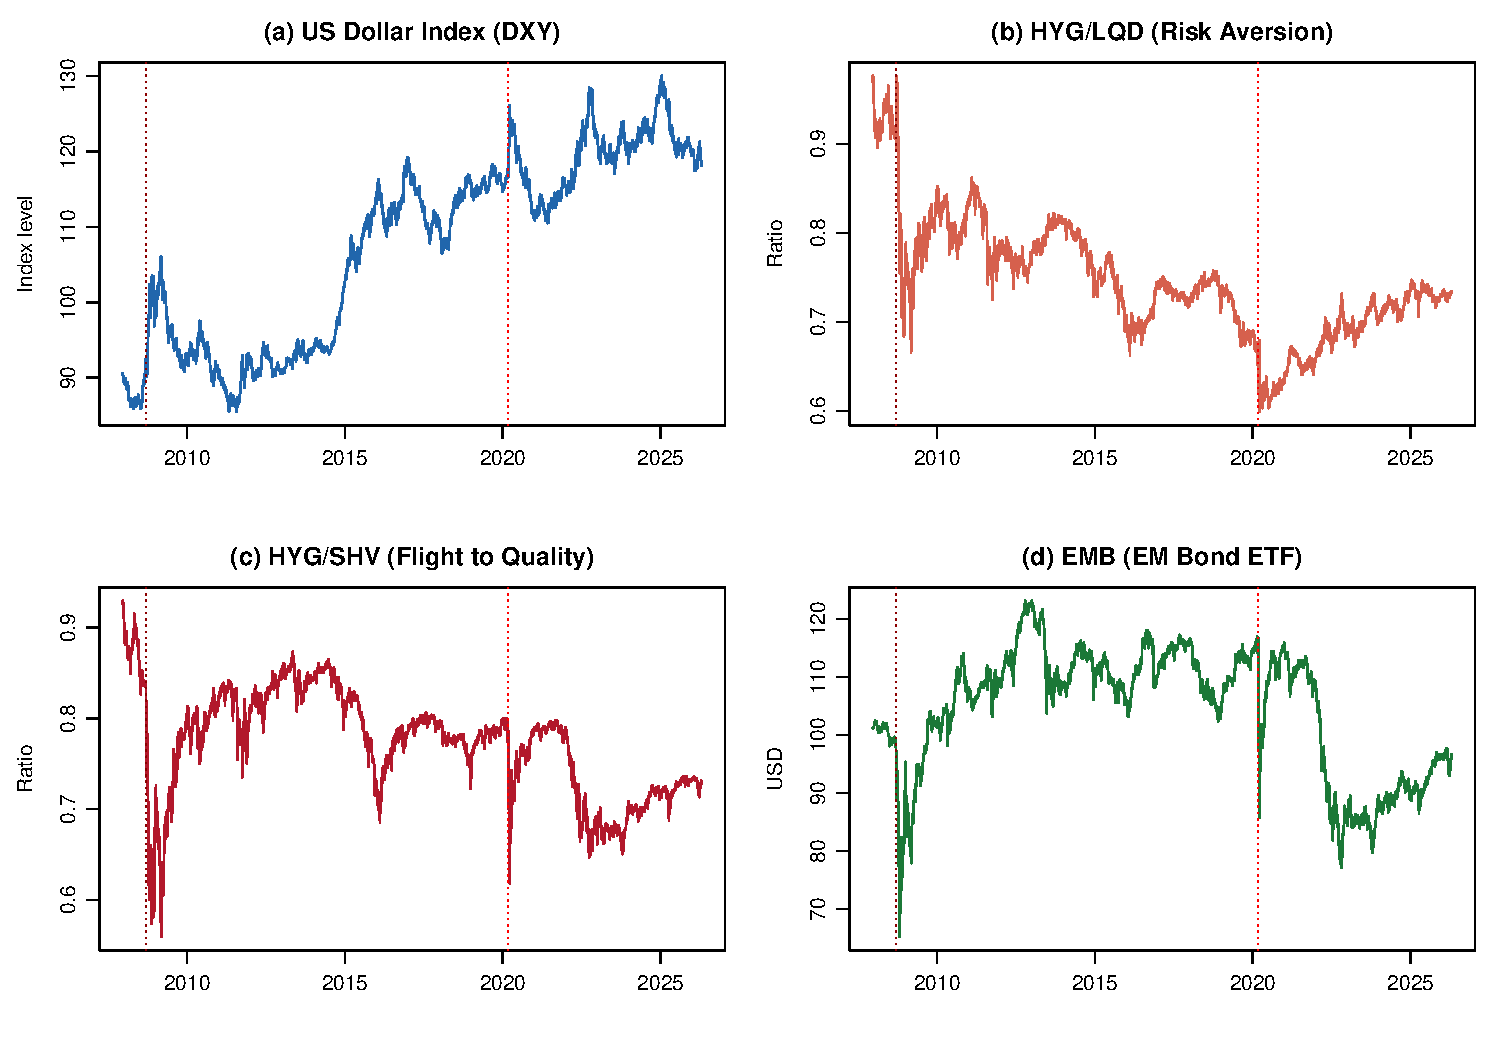
\includegraphics[width=0.95\textwidth]{fig_ts_dollar_credit.pdf}
\caption{Time series of DXY, HYG/LQD ratio, HYG/SHV ratio, and EMB (2008--2026). Dotted lines mark the Lehman collapse and COVID.}
\label{fig:ts_dollar}
\end{figure}


\end{document}
